\section{Introduction}
\label{sec:intro}
Long-context inference has become a critical efficiency bottleneck for LLMs, as autoregressive generation requires dense attention over all preceding context tokens when generating each new token. This makes the cumulative attention cost grow quadratically with context length.
Since many high-performing LLMs are already deployed with dense attention, practice favors inference-efficient methods that avoid architectural changes or retraining.
This motivates post-training attention sparsification\footnote{We use ``post-training'' relative to dense pretraining: it includes methods applied after a dense model has been pretrained, such as mid-training adaptation, post-training fine-tuning, and training-free inference-time sparsification.} 
\citep{tang2024quest, liu2025deepseek, gao2024seerattention, gao2025seerattention}, which adapts dense models into sparse-attention models after pretraining.


\begin{figure}[!t]
    \centering
    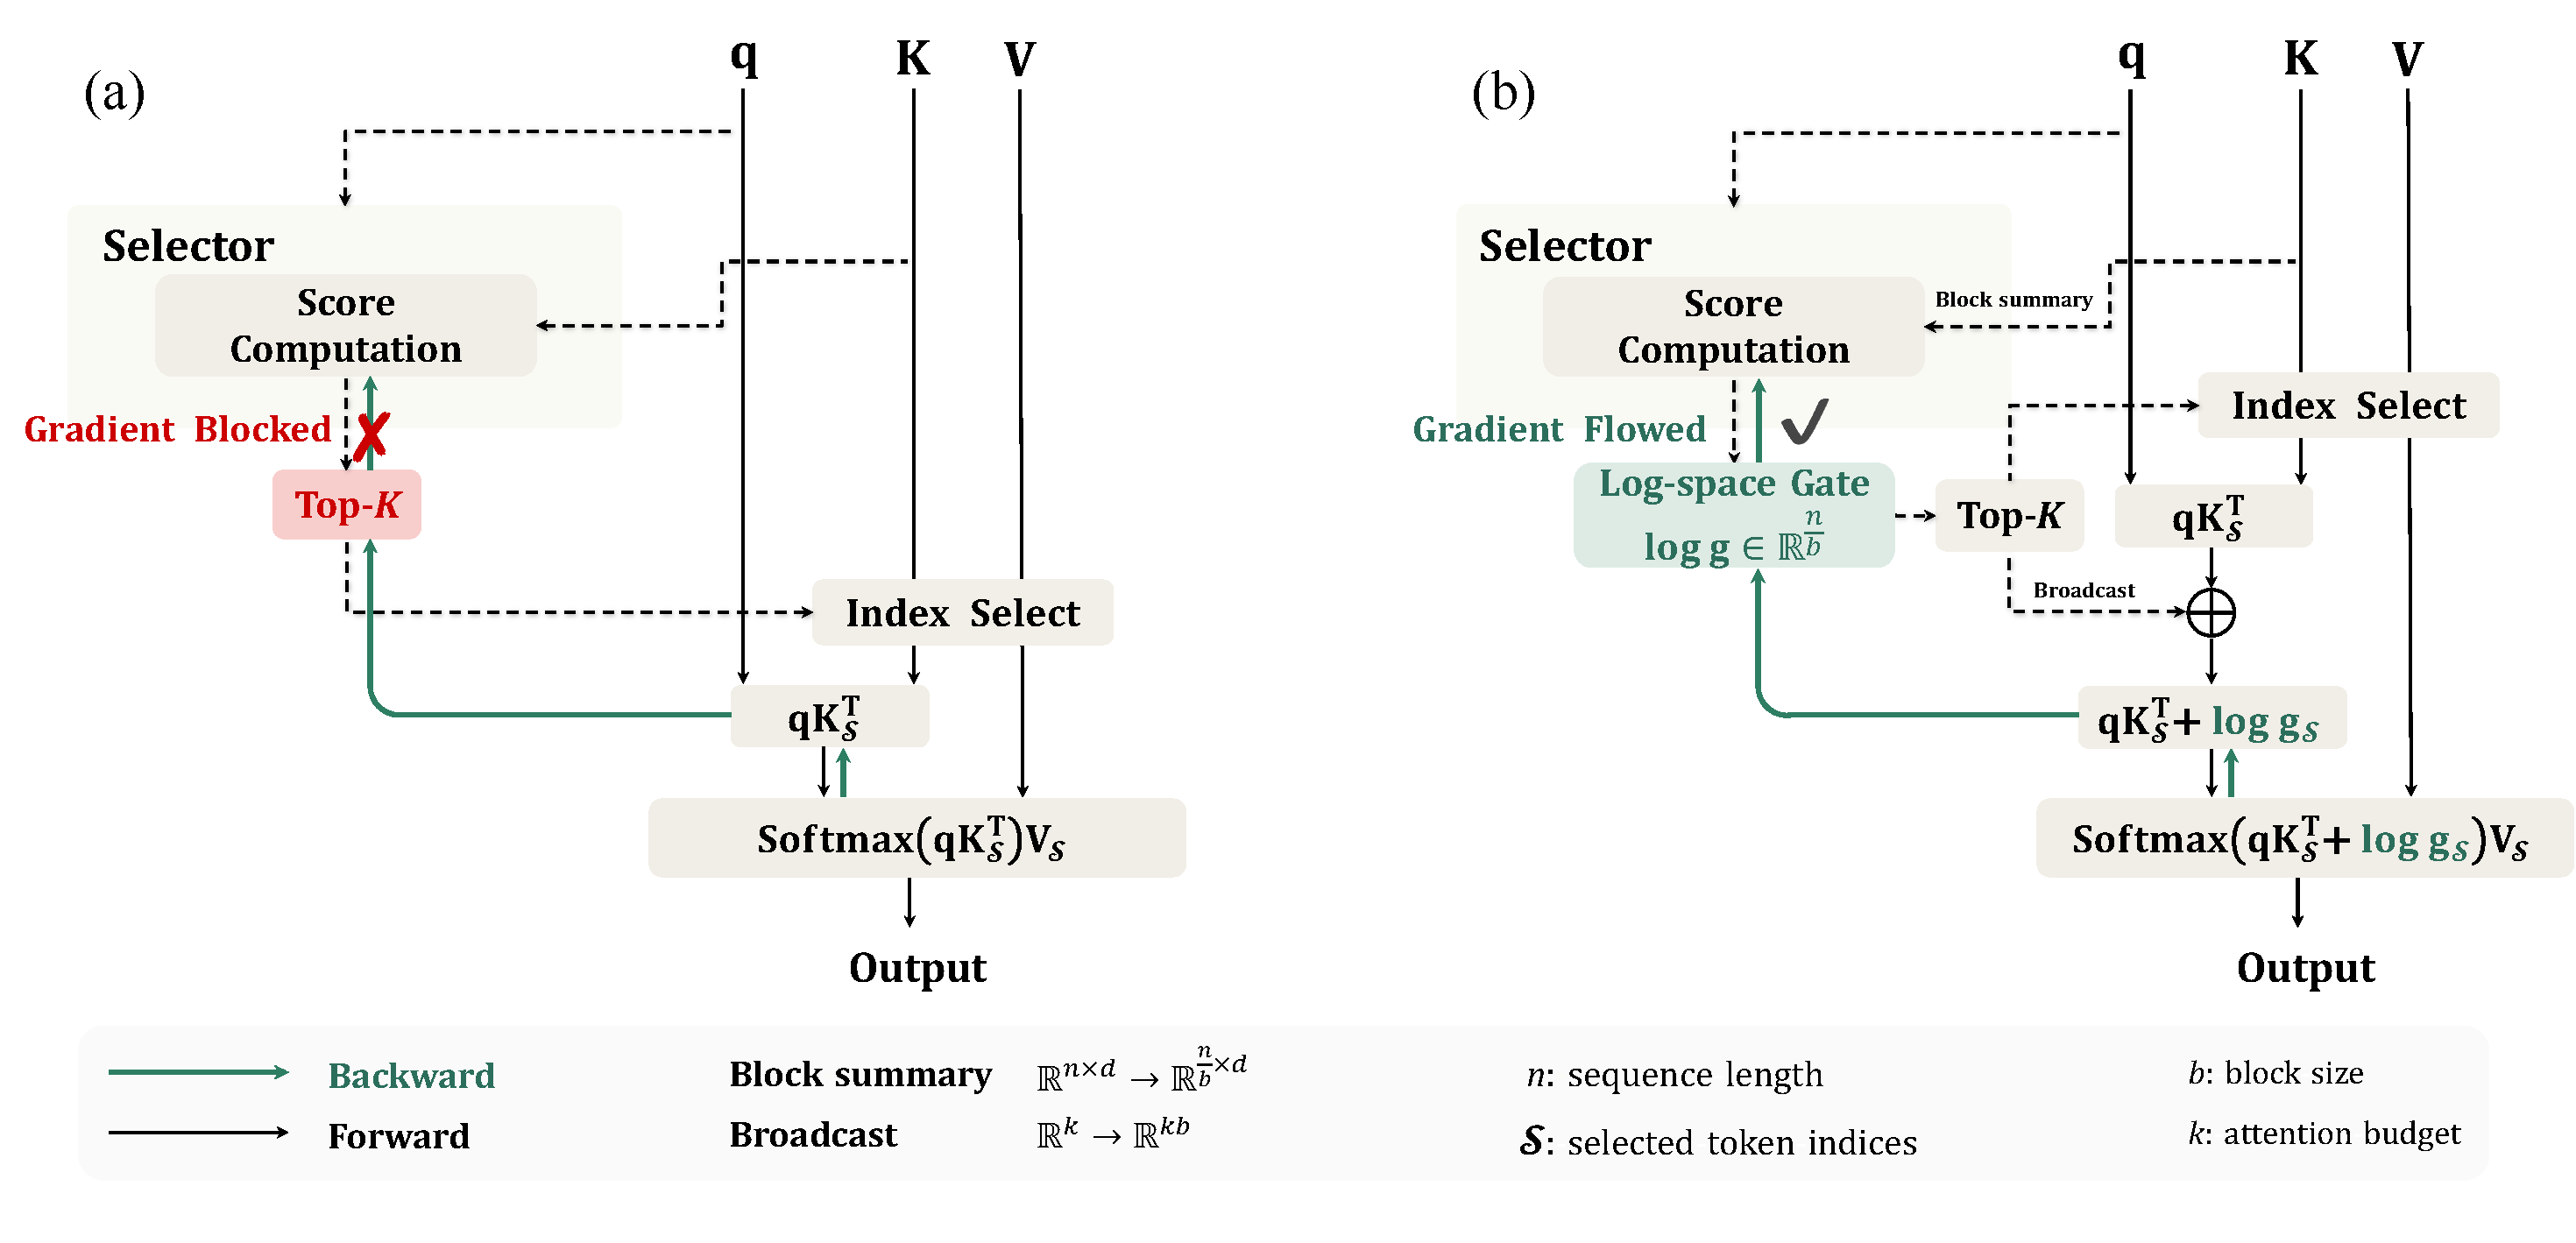
\includegraphics[width=0.99\linewidth]{sec/fig/ours5.pdf}
    \caption{(a) Gradient Blockage in Discrete Selection. Sparse attention with \textbf{discrete Top-$K$ selection} prevents gradients propagation from language modeling loss to selector. Existing approaches bypass this issue using \emph{auxiliary distillation} \citep{deepseekai2026deepseekv4,gao2025seerattention} or \emph{heuristics} \citep{lumoba,zhao2025infllm}. 
    (b) Differentiable Continuous Gating. \our keeps discrete Top-$K$ selection but attaches a continuous soft gate to each selected block, enabling gradient flow from the language modeling loss to the selector.}
    \label{fig:motivation}
\end{figure}

In post-training attention sparsification for LLMs, the central question is how to select the most useful context units (tokens or blocks) for each query under a limited attention budget, where a unit can be an individual token or a coarse-grained block depending on the sparsification scheme.
Many training-free methods address this problem with heuristic or empirical rules~\citep{xiao2023streamingllm,tang2024quest,xiao2024duoattention,lin2025twilight,jiang2024minference}. 
While these training-free methods are attractive for their simplicity, their hand-crafted selection rules cannot adapt the selection strategy to the model's own prediction behavior.
More recently, trainable sparsification has emerged as a promising direction by introducing learnable selectors~\citep{gao2024seerattention,gao2025seerattention,liu2025deepseek}. A selector is a lightweight module that scores context units for each query, after which a hard Top-$K$ step chooses the attended units, enabling a higher performance ceiling than hand-crafted selection rules.
Because hard Top-$K$ selection is non-differentiable, these methods commonly train selectors through layer-wise distillation of dense attention distributions: the selector in each layer is supervised to match the attention mass produced by the original dense model.
However, this surrogate supervision can induce a ranking misalignment: it teaches the selector to rank context units according to where the original dense model attends, rather than by their impact on the model's final predictions under a limited attention budget.
This distillation strategy has two limitations. First, per-layer targets can overlook cross-layer complementarity in context usage. Second, attention matching constrains only attention weights, ignoring how attended \emph{values} (the $\mathbf{V}$ matrix in \Cref{fig:motivation}) affect the final prediction.

In this work, we explore \emph{end-to-end} optimization of context selection with the language modeling loss.
Our key idea is to make the selector's scores part of the differentiable attention computation during training, so that the standard language modeling loss can update the selector through backpropagation.
We instantiate this idea in the open-source block sparse setting of SeerAttention-R~\citep{gao2025seerattention}, where layer-wise selectors score context blocks for each query.
Instead of using layer-wise attention distillation as in SeerAttention-R, we optimize the selectors end-to-end via a simple design: during training, blockwise scores from selector are interpreted as log-space gates, and added to the $\mathbf{q}\mathbf{K}^\top$ attention logits, allowing gradients to flow from the attention computation to the selectors (\Cref{fig:motivation}b).

The effectiveness of this simple design, however, depends on four key choices in how the selector is trained from the language modeling loss.
\emph{(1)} The gate should be added inside the attention $\operatorname{softmax}$ in log form, so selector scores directly modulate attention mass rather than merely rescaling attention outputs.
\emph{(2)} The gate activation should normalize scores across context blocks (\eg, with a $\operatorname{softmax}$), so the gates encode calibrated relative importance rather than unnormalized scores.
\emph{(3)} The selected gates should stay continuous rather than being collapsed into binary Top-$K$ indicators, because the model must learn not only which context blocks are selected but also their relative priorities.
\emph{(4)} Training should update only the selected blocks rather than all context blocks, since it is much cheaper and still reaches comparable final performance.
Together, the first three choices make end-to-end gradients from the language modeling loss informative for learning which context blocks actually support the model's prediction, while the last keeps training efficient.

Besides the design choices above that make the end-to-end optimization effective, we also implement specialized Triton \citep{tillet2019triton} kernels that make long-context training practical. Since a naive implementation would materialize the full attention matrix before adding the log-space gates, which is prohibitive for long-context training, our kernel fuses the gate addition into the tile-level $\mathbf{q}\mathbf{K}^\top$ computation in FlashAttention~\citep{dao2022flashattention}. As a result, attention sparsification with \our is simplified to replacing the attention kernel with our gated-attention kernel and optimizing the standard language modeling loss, without auxiliary distillation.

Despite its simplicity, extensive experiments demonstrate that \our consistently outperforms existing post-training attention sparsification baselines across reasoning, long-context understanding, and agentic tasks. We further provide initial evidence that the same end-to-end optimization applies to continued pretraining, where the backbone and selector are trained jointly.
The improvements are most pronounced under low attention budgets, where accurate context ranking is most critical: on reasoning tasks at a 1024 token budget, \our improves over SeerAttention-R~\citep{gao2025seerattention} by 6.0--7.7 points on MATH500 and 10.6--15.5 points on GPQA-Diamond across Qwen3-4B, 8B, and 14B. The gains extend beyond reasoning: on long-context understanding (LongBench) \our leads SeerAttention-R at every budget, with the largest margins on the longest inputs (\eg, +3.2 on the 8K+ bucket of Qwen3-4B at budget 2048), and on agentic tasks it improves BFCL by up to +3.5 and remains ahead on VitaBench, nearly recovering full attention at budget 4096.
Our contributions are:
{\setlength{\leftmargini}{1.6em}
\begin{itemize}
\item We propose \our, an end-to-end post-training attention sparsification paradigm that trains context selectors with the language modeling loss, removing the need for teacher attention or auxiliary distillation. In controlled comparisons with matched backbones, selector architectures, and training data, \our learns more effective sparse routing than layer-wise attention distillation.
\item 
We identify the design choices that make the simple gated relaxation effective and practical, including log-space gate injection, normalized gate activation, preservation of fine-grained score differences, an efficient sparse training scope, and a memory-efficient kernel for long-context training.
\item 
\our consistently improves performance across reasoning (MATH500, GPQA-Diamond, AIME24, AIME25), long-context understanding (LongBench), and agentic tasks (BFCL, VitaBench), with gains of over 10\% under low attention budgets.
\end{itemize}
}
